\section{Příklad 1}
% Jako parametr zadejte skupinu (A-H)
\prvniZadani{B}

\begin{center}
	{Zjednodušíme schéma pomocí metody trojúhelník - hvězda a napíšeme formuly pomocí Ohmova zákona}
\end{center}

\begin{align*}
	R_A = \frac {R_1 \cdot R_2}{R_1 + R_2 + R_3} = 275,9 \Omega \\
	\\
	R_B = \frac {R_1 \cdot R_3}{R_1 + R_2 + R_3} = 128,5 \Omega \\
	\\
	R_C = \frac {R_2 \cdot R_3}{R_1 + R_2 + R_3} = 144,3 \Omega \\
	\\
	R_{45} = \frac {R_4 \cdot R_5}{R_4 + R_5} = 182,9 \Omega \\
	\\ 
	R_{B457} = \frac {R_1 \cdot R_3}{R_1 + R_2 + R_3} + \frac {R_4 \cdot R_5}{R_4 + R_5} +R_7 = 651,3 \Omega \\
	\\
	R_{C6} = \frac {R_2 \cdot R_3}{R_1 + R_2 + R_3} + R_6 = 974,3 \Omega \\
	\\
	R_{B457C6} =
	\frac
	{( \frac {R_1 \cdot R_3}{R_1 + R_2 + R_3} + \frac {R_4 \cdot R_5}{R_4 + R_5} +R_7) \cdot (\frac {R_2 \cdot R_3}{R_1 + R_2 + R_3} + R_6)}
	{\frac {R_1 \cdot R_3}{R_1 + R_2 + R_3} + \frac {R_4 \cdot R_5}{R_4 + R_5} +R_7 + \frac {R_2 \cdot R_3}{R_1 + R_2 + R_3} + R_6} = 390,4 \Omega 
\end{align*}

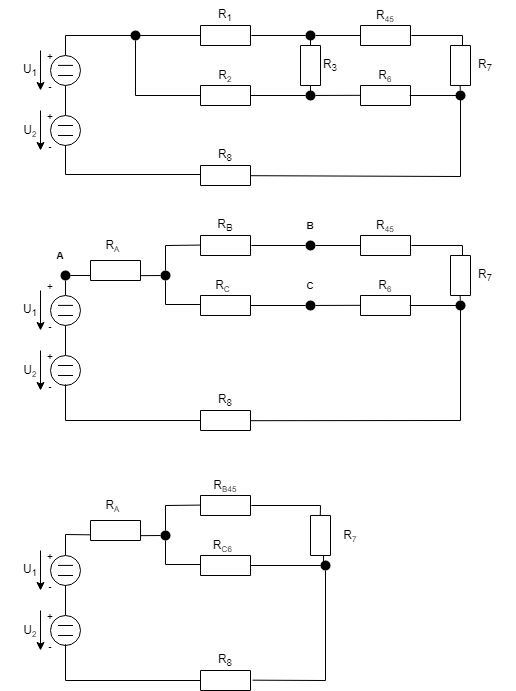
\includegraphics{1.1.png}
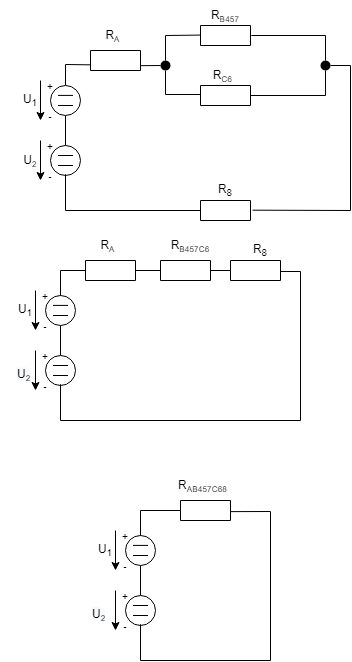
\includegraphics{1.2.png}

\begin{center}
	{Najdeme celkový proud (U najdeme pomocí II. Kirchhoffova zákona)}
\end{center}

\begin{align*}
	 I = \frac {U_{CC}}{R_{ekv}}\qquad
	( R_{ekv} = R_{AB457C6}\qquad U_{CC} = U_1 + U_2 = 210 V) \\
\end{align*}

\begin{center}
	{Teď pomocí vyše napsáných formul můžeme rozepsát celkový proud}
\end{center}

\begin{align*}
	 I = \frac {U_1 + U_2}{  \frac {R_1 \cdot R_2}{R_1 + R_2 + R_3} + 
	\frac
	{( \frac {R_1 \cdot R_3}{R_1 + R_2 + R_3} + \frac {R_4 \cdot R_5}{R_4 + R_5} +R_7) \cdot (\frac {R_2 \cdot R_3}{R_1 + R_2 + R_3} + R_6)}
	{\frac {R_1 \cdot R_3}{R_1 + R_2 + R_3} + \frac {R_4 \cdot R_5}{R_4 + R_5} +R_7 + \frac {R_2 \cdot R_3}{R_1 + R_2 + R_3} + R_6} + R_8 } = 0,237 A\\
\end{align*}

\begin{center}
	{Najdeme $U_{R_{B457}} $ (on je zapojen paralelně s $U_{R_{C6}}$ (viz obr. na straně 4) a potom $I_{R_{B457}}$, takže bude platit: }
\end{center}

\begin{align*}
	U_{R_{B457}} = U_{R_{C6}} = U_{CC} - U_{R_{A}} - U_{R_{8}}\\
	U_{R_{A}} = R_{A} \cdot I = 65,38 V\\
	U_{R_{8}} = R_{8} \cdot I = 52,14 V\\
	\\
	U_{R_{B457}}  = 92,5 V\\
	\\
	\underline{ I_{R_{B457}} = \frac {U_{R_{B457}}}{R_{B457}} = 0,142 A = I_{R_{7}}}\\
	\\
\end{align*}

\begin{center}
	{Dle Ohmova zákona: }
\end{center}

\begin{align*}
	\underline{U_{R_{7}} = I_{R_{7}} \cdot R_{7} = 48,1 V}
\end{align*}

